The XtreemFS client connects applications to XtreemFS and acts as a gateway to the XtreemFS directory (DIR), metadata (MRC\index{MRC}), and object store (OSD\index{OSD}) servers. From a user's perspective, the client consists of a number of binary programs that reside on the user's machine. These programs and their functions are summarized in table \ref{xtreemfs_client/tables/command_line_tools}.

\begin{table}[!h]
\begin{tabularx}{\linewidth}{|l|X|}
\hline
Command line tool & Function \\
\hline
\texttt{xtfs\_lsvol} & list volumes on an XtreemFS MRC\index{MRC} server \\
\texttt{xtfs\_mkvol} & create a volume on an XtreemFS MRC\index{MRC} server \\
\texttt{xtfs\_mount} & mount an XtreemFS volume  \\
\texttt{xtfs\_rmvol} & delete a volume on an XtreemFS MRC\index{MRC} server \\
\texttt{xtfs\_send} & send arbitrary RPCs to an XtreemFS server \\
\texttt{xtfs\_stat} & print statistics on an XtreemFS file or directory \\
\hline
\end{tabularx}
\caption{XtreemFS client command line tools}
\label{xtreemfs_client/tables/command_line_tools}
\end{table}

\subsection{Architecture}

The client is structured as a network of message-processing \textit{stages} connected by queues. These stages are similar to those in the XtreemFS servers, and are designed with the same intent: to increase concurrency while avoiding data races (see \cite{SEDA} and previous deliverables for an explanation of stages). Unlike the XtreemFS servers, which is implemented in Java and uses a custom-built set of classes for managing stages, the client is implemented in C++ and relies on a third party platform, Yield \footnote{\url{http://yield.googlecode.com/}} for much of its low-level functionality, including concurrency control in the form of stages as well as platform-specific primitives such as files and sockets.

The stage architecture of the XtreemFS client is depicted in figure \ref{xtreemfs_client/figures/xtreemfs_client_stages}. Note that this particular configuration of stages is specific to \texttt{xtfs\_mount}, which consists of a set of FUSE\index{FUSE} entry points and proxy stages for the various XtreemFS servers with which \texttt{xtfs\_mount} communicates: the directory server (\texttt{DIRProxy}), the metadata server (\texttt{MRCProxy}), and one or more object stores (\texttt{OSDProxy}).

\begin{figure}[htbp]
\centering
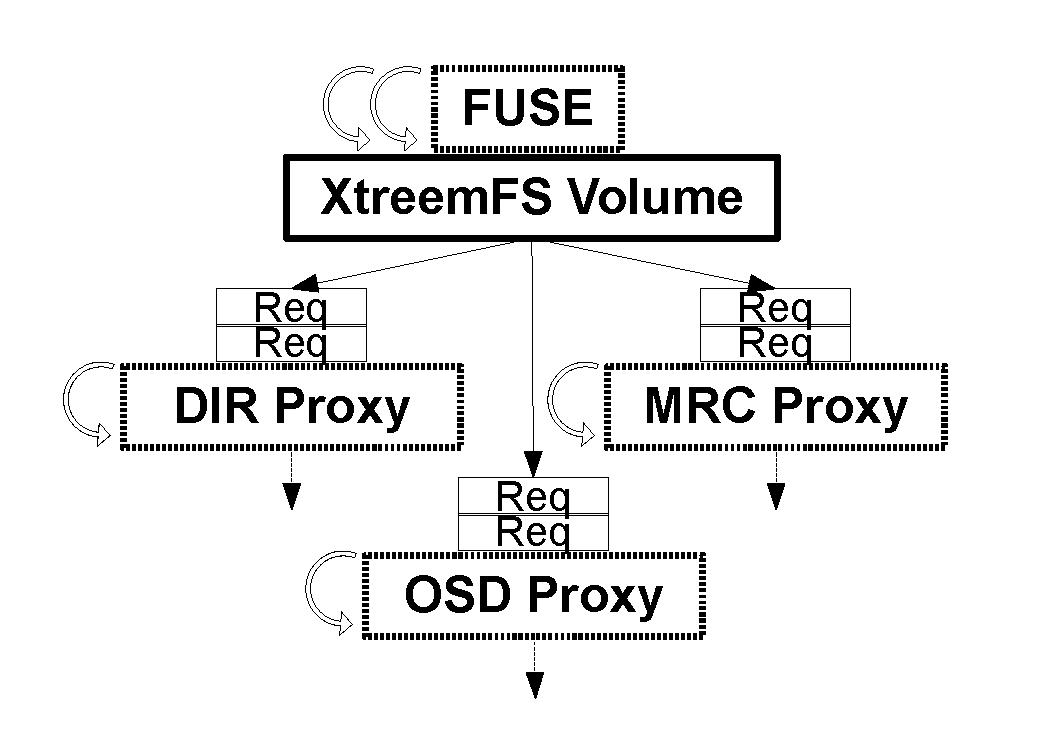
\includegraphics[width=.80\columnwidth]{images/xtreemfs_client_stages}
\caption{Client stages}
\label{xtreemfs_client/figures/xtreemfs_client_stages}
\end{figure}

\subsubsection{FUSE\index{FUSE}}

\texttt{xtfs\_mount} provides a file system interface to applications via FUSE\index{FUSE} \footnote{\url{http://fuse.sourceforge.net/}}, a library for implementing file systems in userspace. Applications make POSIX\index{POSIX} system calls such as \texttt{open} and \texttt{read} into the operating system kernel. A FUSE\index{FUSE} kernel module translates these calls into messages (i.e. Remote Procedure Calls), which are then passed to a FUSE\index{FUSE} file system via a pipe. The file system runs as a daemon in an infinite loop, reading and processing messages from the pipe and sending responses back into the kernel. The userspace part of the FUSE\index{FUSE} library handles most of the nitty gritty details of kernel-userspace communication, so that the file system implementator can concentrate on implementing file system logic. This is typically done by implementing a set of FUSE\index{FUSE} callbacks, each of which corresponds to a POSIX\index{POSIX} system call (and thus a message on the FUSE\index{FUSE} pipe as well). The FUSE\index{FUSE} library translates messages to calls on the callbacks supplied by the file system developer and translates return values from the callbacks back into messages for the FUSE\index{FUSE} kernel module. These FUSE\index{FUSE} callbacks are the main entry points into \texttt{xtfs\_mount}.

From a FUSE\index{FUSE} callback such as \texttt{mkdir} the client makes a series of requests (messages) through the various stages shown in figure \ref{xtreemfs_client/figures/xtreemfs_client_stages}. The primary stages in the client are proxies for the servers the \texttt{xtfs\_mount} instance is connected to: typically a single DIR server and a single MRC\index{MRC} server and multiple OSD\index{OSD} servers. In the case of \texttt{mkdir} the client would send a request to the \texttt{MRCProxy} to create the specified directory. Because the FUSE\index{FUSE} callbacks are synchronous the initial request from a callback to a stage must be synchronous, i.e. the sender must wait for the response before doing any further processing. However, this does not mean that the whole system is synchronous: only the FUSE\index{FUSE} callback blocks synchronously on a request, allowing the stages in the client to communicate asynchronously (and thus improve performance). Furthermore, since the FUSE\index{FUSE} callbacks may be multithreaded and reentrant a stage (such as e.g. the \texttt{MRCProxy}) can process requests from multiple FUSE\index{FUSE} callbacks simultaneously. In other words, the concurrency of the client is not limited by the FUSE\index{FUSE} front end and the number of threads processing FUSE\index{FUSE} messages.

\subsection{Implementation}

The XtreemFS client is implemented entirely in C++. Aside from the essential components listed above (FUSE\index{FUSE} callbacks, server proxies) \texttt{xtfs\_mount} consists of a few support classes such as \texttt{Path} (which wraps XtreemFS \texttt{volume\/file} global paths) and XtreemOS integration code such as a pluggable module for retrieving user credentials from an XtreemOS AMS server. Most of this code is shared between the XtreemFS command line tools listed in table \ref{xtreemfs_client/tables/command_line_tools}. As mentioned previously, the XtreemFS client also relies heavily on Yield for many low-level classes, such as platform-specific file paths and sockets. The ONC-RPC \cite{RFC1831} protocol implementation used to communicate with the XtreemFS servers is also a part of Yield. 

\subsubsection{Generated interfaces}

The synchronous request-response messages exchanges between FUSE\index{FUSE} callbacks and stages such as the \texttt{MRCProxy} are hidden underneath a function call interface. The latter is generated from the same IDL\index{IDL} interfaces used by the server. When one of the interface operations is called synchronously on the \texttt{MRCProxy} a request is created and filled with the function parameters; the request is sent to the \texttt{MRCProxy} stage, where it is processed asynchronously; and the caller blocks waiting for the response, which, when it is received, is unpacked and returned as a normal function return value. The extra level of abstraction allows the FUSE\index{FUSE} callback interface to be fully agnostic of message sending and receiving, and simply treat the MRCProxy as if it were making synchronous remote procedure calls. The FUSE\index{FUSE} callback for \texttt{mkdir} is shown in figure \ref{xtreemfs_client/figures/xtreemfs_client_mkdir_code}.

\begin{figure}[h!]
\begin{verbatim}
bool Volume::mkdir( const YIELD::Path& path, mode_t mode )
{
  mrc_proxy.mkdir( Path( this->name, path ), mode );
  return true;
}
\end{verbatim}
\caption{FUSE\index{FUSE} callback for mkdir}
\label{xtreemfs_client/figures/xtreemfs_client_mkdir_code}
\end{figure}

\subsubsection{Lines of code}

With much of its low-level functionality in Yield and other libraries the code base for the XtreemFS client is quite minimal, with approximately 2800 lines of hand-written C++ and 4800 lines of C++ automatically generated from the XtreemFS IDL\index{IDL} interfaces.